\chapter{Methods}
\label{chap:methods}

This chapter describes the methodology used to develop and evaluate the proposed vehicle detection and tracking pipeline, summarized in \autoref{fig:tech_workflow}. Video streams were collected from two SVV traffic camera stations across multiple times of day and weather conditions. A diverse set of frames was extracted and semi-automatically annotated, then partitioned into training, validation, and test splits before fine-tuning YOLO26n and YOLO26m. The trained detectors were subsequently combined with multiple MOT configurations, including ByteTrack, standard BoT-SORT, and two custom BoT-SORT variants optimized for daytime and nighttime conditions, and evaluated using a zone-based Origin--Destination framework on manually annotated clips. A dedicated day--night transition sequence was additionally used to demonstrate continuous operation under changing illumination.

\begin{figure}[H]
    \centering
    \includegraphics[width=1\linewidth]{project//images/tech_workflow4.png}
    \caption[Overall technical workflow of the custom vehicle detection and tracking pipeline]{Overall technical workflow of the custom vehicle detection and tracking pipeline developed in this thesis.}
    \label{fig:tech_workflow}
\end{figure}


\section{Data Description and Dataset Preparation}
This section describes the data source and acquisition process, summarizes data quality constraints, and details the annotation workflow and dataset partitioning used for model development and evaluation.

\subsection{Data Source and Acquisition}
The Norwegian Public Roads Administration operates 783 publicly accessible traffic camera stations across Norway. However, the majority of these stations provide only still images captured at ten-minute intervals and do not record continuous video streams. Among the limited number of stations that offer live video feeds, only a small subset is situated in intersections.

Two relevant camera stations were identified, with the first being mounted at Fv587 Haukeland, Bergen (Direction Arna), which is shown in \autoref{fig:haukeland_bilde}. The intersection is an unsignalized T-intersection, where a secondary road connects to the main road. Marked pedestrian crossings are present across the main approaches, and a bus bay with a sheltered stop is located along both roadsides. The area around the intersection includes a small number of residential buildings, open land, and roadside vegetation.

The second relevant camera station is mounted at Rv36 Kjørbekk (direction Porsgrunn), which is shown in \autoref{fig:kjørbekk_bilde}. The intersection is also an unsignalized T-intersection where a secondary road connects to the main road. Towards the top of the frame, the main road leads into a roundabout that facilitates traffic distribution in various directions. A pedestrian and bicycle path runs parallel to the main road on the right side. Near the T-intersection, an underground pedestrian crossing allows individuals to safely cross beneath the main road. Additionally, a bus stop is located along the roadside on the left.

\begin{figure}[H]
     \centering
     \begin{subfigure}[b]{0.48\textwidth}
         \centering
         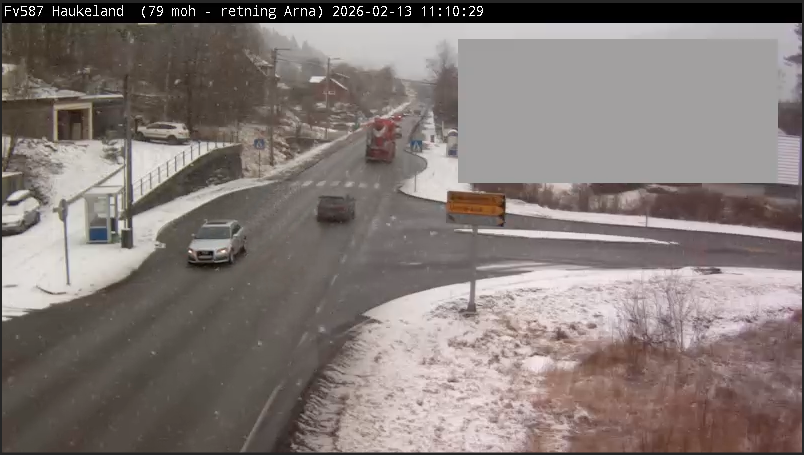
\includegraphics[width=\linewidth]{project/images/haukeland_bilde.png}
         \caption{Fv587 Haukeland}
         \label{fig:haukeland_bilde}
     \end{subfigure}
     \hfill
     \begin{subfigure}[b]{0.48\textwidth}
         \centering
         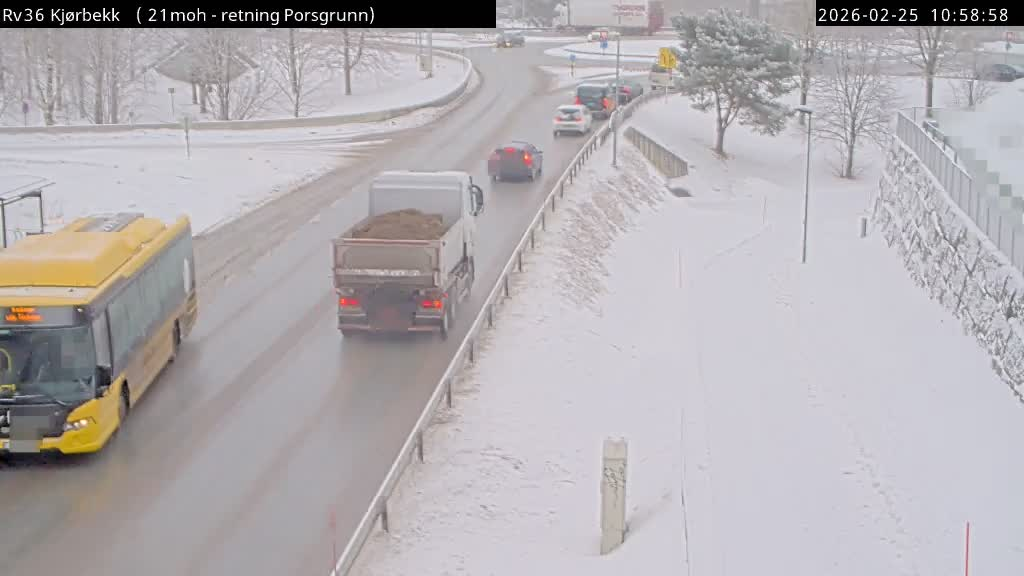
\includegraphics[width=\linewidth]{project/images/kjørbekk_bilde.jpg}
         \caption{Rv36 Kjørbekk}
         \label{fig:kjørbekk_bilde}
     \end{subfigure}
     \caption{Snapshots of video streams at different camera stations. Source: \cite{SVV_HaukelandKamera}}
     \label{fig:combined_cameras}
\end{figure}

The video data was captured from the SVV live streams using an FFmpeg script targeting the m3u8-stream URLs (Appendix~\ref{app:ffmpeg}). To manage the data efficiently, the continuous streams were segmented into five-minute MPEG-4 video clips. Rather than using the entire raw video duration, a strategic sampling approach was implemented to maximize the quality and relevance of the dataset.

Initially, frames were extracted at random intervals to establish a baseline. However, as the base YOLO26 model is pre-trained on the COCO dataset, it already possessed high proficiency in identifying standard passenger cars. To focus the training on specialized vehicle classes, the strategy shifted toward manual frame extraction, specifically targeting intervals containing heavy vehicles.

As the custom model’s weights were updated and its performance improved, a more automated model-in-the-loop approach was introduced. A custom script was developed to process the video segments, running the current YOLO weights on every frame and automatically extracting only those images where the model detected heavy vehicles. This filtering process significantly reduced the redundancy of the dataset, ensuring that the manual annotation effort was concentrated on the most informative samples for the model's specific objectives. This process resulted in a final dataset of 1282 images.


\subsection{Data Quality and Limitations}

The video data varies in resolution and frame rates between the two recording sites. The stream from Fv587 Haukeland is captured at a resolution of 800 × 450 pixels. During the data collection period, this stream was delivered at approximately 10 FPS (7 FPS at night) and contained a large grey censoring box in the upper right corner. As of April 13$^{th}$ 2026, the grey box has been removed, the frame rate has been doubled, and the field of view has been slightly zoomed out. The Rv36 Kjørbekk station provides a higher spatial resolution of 1024 × 576 pixels, but at a lower frame rate of roughly 5 FPS. To ensure the model's robustness and ability to generalize, the dataset was extracted at various times of the day, encompassing a wide range of weather conditions, from clear daylight to dark, foggy, and snowy environments, as illustrated in \autoref{fig:weather_conditions}. This diversity in the training data is crucial for the model to accurately identify vehicles despite shifting shadows, varying light intensity, and reduced visibility due to precipitation.

\begin{figure}[H]
    \centering
    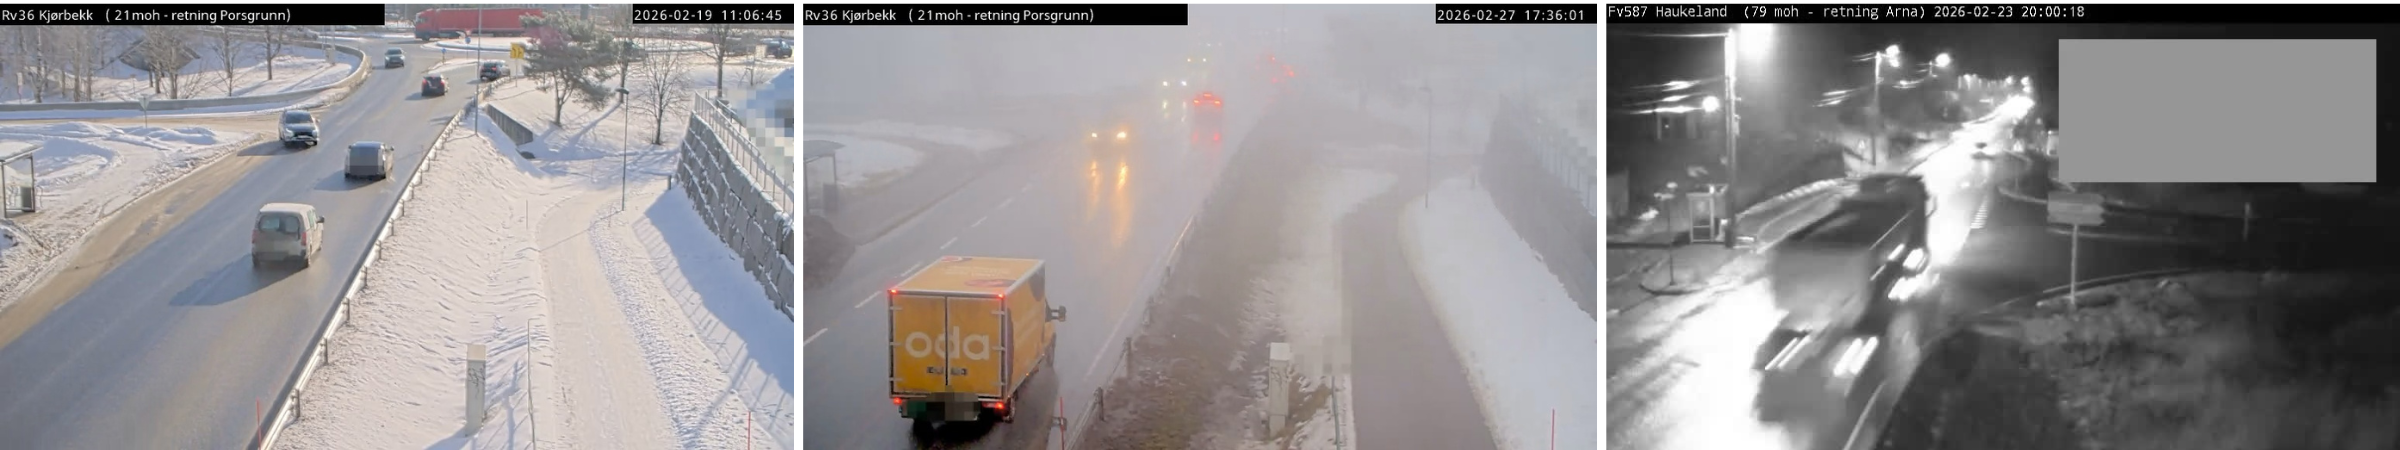
\includegraphics[width=1\linewidth]{project/images/weather_conditions.png}
    \caption[Examples of environmental and lighting variations in the dataset]{Examples of environmental and lighting variations in the dataset. Source: \cite{SVV_HaukelandKamera}}
    \label{fig:weather_conditions}
\end{figure}

The data acquisition process was subject to several constraints that shaped the final composition of the dataset. Since SVV does not provide access to historical video archives, the study relied exclusively on live-stream captures. This prevented the retrieval of data from different seasons or specific past traffic events, effectively tying the dataset to the environmental conditions present during the recording period. Consequently, because the recordings were conducted during the Norwegian winter/early spring, the dataset reflects a notable scarcity of pedestrians, cyclists, and motorcyclists. Furthermore, the relatively low traffic volume at the selected sites necessitated extended recording periods to ensure a sufficient number of observations for the less frequent vehicle classes.

A significant technical limitation is the automated privacy masking implemented by SVV on their public live streams. To comply with privacy regulations, the system is designed to blur or pixelate license plates and faces. In practice, this masking introduces image artifacts and removes fine-grained texture information, which can reduce classification reliability for visually similar vehicle categories. Moreover, because the masking can change abruptly between frames, it can degrade appearance-based association in multi-object tracking and increase the risk of ID switches. In many instances, particularly at the Rv36 Kjørbekk station, this automated censorship is overly aggressive, occasionally causing the entire vehicle to become heavily pixelated. This loss of visual data poses a challenge for both manual annotation and model training.

This technical challenge is further compounded by the subjective nature of manual classification. As the annotators are not professional vehicle experts, certain edge cases proved difficult to categorize with absolute certainty. Visual ambiguity, often made worse by distance, poor weather conditions or pixelation, introduces a margin of human error in the labeling process. These inconsistencies in the ground-truth data may impact the model’s ability to learn the fine-grained distinctions required to accurately differentiate between visually similar vehicle configurations.


\subsection{Data Annotation}
\label{sec:data_annotation}
To address the research gap identified in Section~\ref{sec:research_gap}, where most existing automatic vehicle detection studies are limited to a small number of standard vehicle classes and fail to capture the full diversity of real-world road users \citep{Maity2022LastDecadeVehicleDetection}, the development of the custom object detection model follows an iterative, semi-automated annotation pipeline specifically designed to incorporate a broader and more granular set of vehicle classes.

As shown in \autoref{fig:annotation_workflow}, the process begins by defining the target vehicle classes, followed by an initial pre-annotation phase. To ensure a consistent and reproducible labeling environment, Label Studio was deployed using Docker, allowing for seamless integration of the annotation interface with custom backend scripts. A subset of images is initially processed using a base YOLOv8 model to generate preliminary labels. These are then manually reviewed within Label Studio to adjust bounding boxes, correct misclassifications, and incorporate ``non-COCO'' classes, such as \textit{light truck}, \textit{heavy truck}, and \textit{semi-trailer / combination vehicle}. Once a high-quality initial dataset is established, it is used to train a custom model. This trained model is subsequently deployed to pre-annotate new image batches, after which human annotators perform final manual corrections. This approach ensures high ground-truth accuracy while significantly reducing the time required to expand the dataset.

\begin{figure}[H]
    \centering
    \includegraphics[width=1\linewidth]{project/images/annotation-workflow.png}
    \caption{Annotation workflow diagram.}
    \label{fig:annotation_workflow}
\end{figure}

\subsubsection*{Annotation Rules and Class Definitions}
To ensure consistency and reduce ambiguity, vehicles were categorized based on physical characteristics and axle counts. Objects at extreme distances or those with insufficient visibility were excluded from the dataset to prevent the model from learning from ambiguous features. \autoref{fig:classes} visualizes the classes that are described below.

\begin{itemize}
    \item \textbf{Car}: Includes all standard passenger vehicles, including sedans, SUVs, and commercial vans.
    \item \textbf{Bus}: Includes public transit buses and other buses.
    \item \textbf{Light Truck}: Two-axle commercial and delivery vehicles, including passenger cars towing small trailers, whose length and weight profiles are more consistent with light freight vehicles than private cars. Tractors and camping vans are also included in this category.
    \item \textbf{Heavy Truck}: Rigid trucks with three axles. In addition, Semi-trailer tractor units (bobtails) traveling without a trailer are included.
    \item \textbf{Semi-trailer / Combination Vehicle}: Includes all articulated vehicles with four or more axles.
    \item \textbf{Motorcycle}: Includes both high-capacity motorcycles and small-engine scooters.
    \item \textbf{Bicycle}: Includes all human-powered or electric bicycles.
    \item \textbf{Person}: Includes individual pedestrians and stationary persons within the traffic environment.
\end{itemize}

\begin{figure}[H]
    \centering
    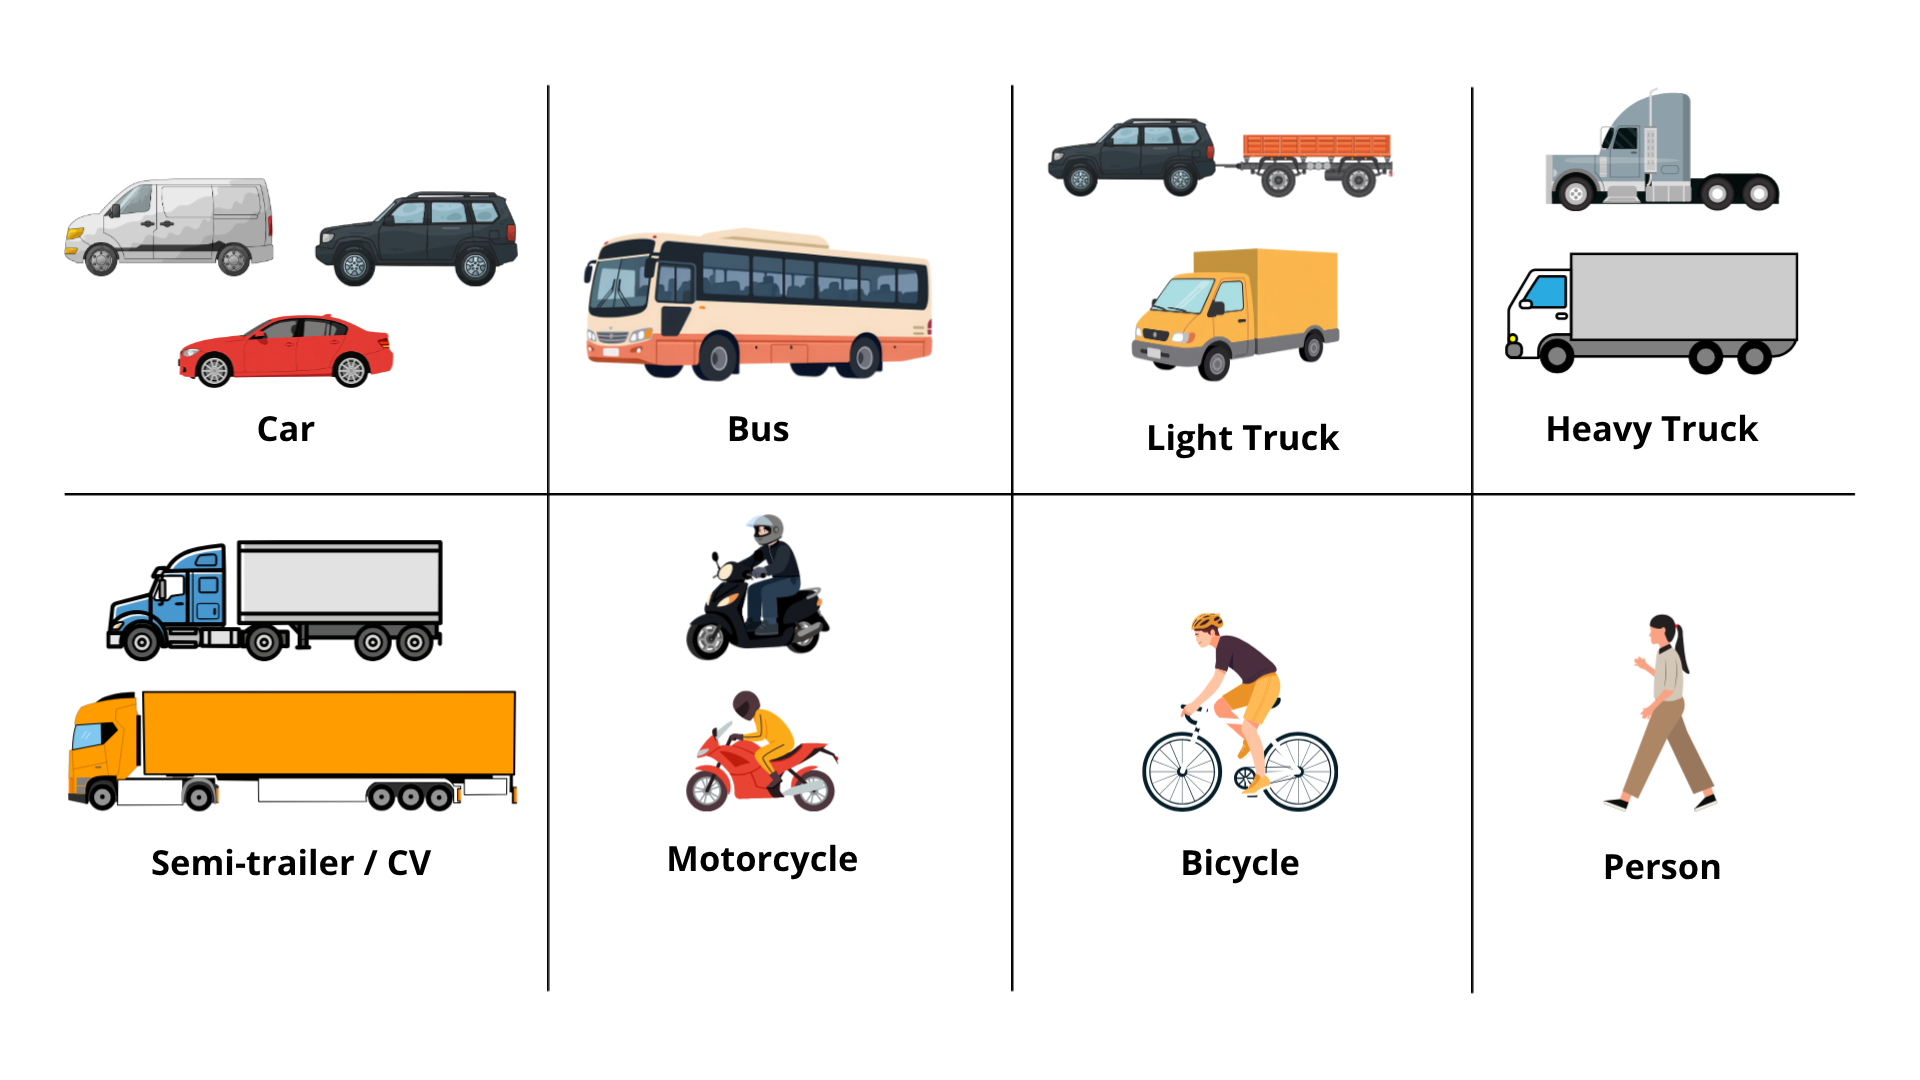
\includegraphics[width=0.8\linewidth]{project//images/classes.png}
    \caption{Visualization of the 8 classes in the dataset.}
    \label{fig:classes}
\end{figure}

\subsection{Dataset Partitioning}
Scikit-learn was used to partition the 1282 annotated images using a randomized 70/15/15 split into training, validation, and test subsets (\autoref{fig:tvt_split}). The training set was used to optimize model weights, while the validation set was used to monitor generalization during training, apply early stopping, and select the best-performing checkpoint. The test set was held out throughout training and was used only once for the final evaluation of the selected model, providing an unbiased estimate of performance on unseen data.

\begin{figure}[H]
    \centering
    \includegraphics[width=0.75\linewidth]{project//images/tvt_split.png}
    \caption{Train/Validation/Test Split}
    \label{fig:tvt_split}
\end{figure}


\section{Model Selection}
Following the theoretical evaluation of modern object detection architectures in \autoref{sec:computer_vision}, YOLO26 was selected as the core framework for this study. Based on the performance metrics summarized in \autoref{tab:yolo26-sizes}, this study evaluates two specific versions of the YOLO26 architecture to address the trade-off between computational efficiency and detection precision.

\begin{itemize}
   \item \textbf{YOLO26n (Nano):} Selected for its high CPU efficiency, achieving 26\,FPS (ONNX Runtime) on standard hardware. To evaluate practical feasibility, YOLO26n is therefore paired with the most lightweight tracker configuration and benchmarked end-to-end on CPU for the complete pipeline.

   \item \textbf{YOLO26m (Medium):} Chosen as the high-performance benchmark. The large (l) and extra-large (x) variants were excluded due to higher computational demands with diminishing returns relative to YOLO26m for our deployment-oriented setting.
\end{itemize}

\begin{table}[H]
\centering
\small
\caption[Ultralytics YOLO26 detection performance metrics on COCO val2017]
{Ultralytics YOLO26 detection performance metrics on COCO val2017. Adapted from \cite{sapkota2026yolo26keyarchitecturalenhancements}.}
\label{tab:yolo26-sizes}
\begin{tabular}{@{}lrrrrrr@{}}
\toprule
Model & \makecell{mAP$^{50-95}$ \\ (e2e)} & \makecell{Speed CPU \\ ONNX (ms)} & \makecell{Speed T4 \\ TRT10 (ms)} & \makecell{FPS CPU \\ (approx.)} & \makecell{FPS T4 \\ (approx.)} & \makecell{Params \\ (M)} \\
\midrule
YOLO26n & 40.1 & 38.9 & 1.7 & 26 & 588 & 2.4 \\
YOLO26s & 47.8 & 87.2 & 2.5 & 11 & 400 & 9.5 \\
YOLO26m & 52.5 & 220.0 & 4.7 & 4.5 & 213 & 20.4 \\
YOLO26l & 54.4 & 286.2 & 6.2 & 3.5 & 161 & 24.8 \\
YOLO26x & 56.9 & 525.8 & 11.8 & 1.9 & 85 & 55.7 \\
\bottomrule
\end{tabular}
\end{table}

\subsection{Training Configuration and Hyperparameters}
The selected YOLO26n and YOLO26m models were fine-tuned in Google Colaboratory using an NVIDIA Tesla T4 GPU and Python 3.12.12. The detection architecture was implemented via the Ultralytics (v8.3.0) framework.

Each model was trained for 100 epochs using an input image size of 640 pixels and a batch size of 16. To optimize training efficiency and prevent overfitting, an early-stopping patience of 20 epochs was implemented, which terminates the process if no improvement is detected in the validation metrics. The model’s weights are initialized from COCO-pretrained checkpoints.

The training of the model was conducted using the default hyperparameter configurations provided by the YOLO26 framework (Appendix~\ref{app:hyperparameters}). Traditionally, achieving optimal performance in object detection requires iterative "tuning sessions," where the model is retrained multiple times to find the best combination of variables. In this study, no manual hyperparameter tuning was performed, as this process is both time-consuming and computationally expensive, particularly under the resource constraints of a Google Colab Tesla T4 GPU environment. The default training configuration also includes data augmentation techniques, such as mosaic augmentation, HSV color jitter and horizontal flipping. To improve reproducibility across runs, the random seed was fixed to 42, ensuring consistent stochastic behavior. 

Additionally, the architectural advancements in YOLO26 significantly mitigate the necessity for such extensive tuning. By utilizing an NMS-free design, the requirement to manually optimize IoU and confidence thresholds is entirely removed. Furthermore, the implementation of the MuSGD optimizer provides a more robust and stable learning process than the SGD or AdamW optimizers used in models ranging from YOLOv8 to YOLOv11, which required extensive hyperparameter tuning \citep{sapkota2026yolo26keyarchitecturalenhancements}.

\section{Multi-Object Tracking for Origin-Destination Estimation}
\label{sec:method_tracking_od}

After fine-tuning YOLO26 on the SVV intersection dataset, the resulting custom-trained YOLO26n and YOLO26m models are used as the detection backbone in the full video-processing pipeline. While object detection provides per-frame bounding boxes and vehicle class predictions, the extraction of traffic engineering parameters such as turning movements requires consistent vehicle identities over time. Therefore, multi-object tracking is applied to associate detections across consecutive frames and reconstruct vehicle trajectories through the intersection.

Building on these trajectories, an origin--destination (O--D) estimation procedure is implemented to assign each tracked vehicle an entry approach (origin) and an exit approach (destination) based on predefined spatial gate regions. This enables automated estimation of turning movements and directional traffic volumes, which are later compared against manual ground-truth counts for validation.

\subsection{Tracking Algorithm}
\label{sec:method_tracker}

Multi-object tracking is performed using the tracking algorithms available in the Ultralytics YOLO framework. The implementation evaluates these different trackers: ByteTrack, standard BoT-SORT, and two custom BoT-SORT configurations optimized for daytime and nighttime conditions, respectively.

All trackers are applied in track mode with persistent identities enabled, allowing each detected vehicle to be assigned a consistent track ID across frames. ByteTrack serves as a lightweight baseline for performance comparison, while BoT-SORT is employed for its ability to incorporate appearance-based re-identification (ReID). However, the production pipeline employs an adaptive approach: a custom BoT-SORT configuration is selected dynamically based on detected lighting conditions, as detailed in Section~\ref{sec:method_dynamic_switching}.

In addition to the default implementations, custom BoT-SORT configurations are deployed to improve tracking robustness in traffic scenarios. For daytime operations, the configuration is specified in \textit{day\_botsort.yaml}. For night-time operations, a conservative configuration file \textit{night\_botsort\_conservative.yaml} is used to handle low-light conditions and headlight-induced artifacts while minimizing false track associations. 

Table~\ref{tab:botsort-config} summarizes the parameters used in both configurations. Compared with daytime settings, the conservative night profile uses stricter association criteria and a substantially larger track buffer to reduce ID fragmentation and false associations in low-light scenes. Appearance-based ReID is enabled in the daytime configuration to leverage visual cues for re-association, but disabled at night where those cues are less reliable.

\begin{table}[H]
\centering
\small
\setlength{\tabcolsep}{8pt}
\renewcommand{\arraystretch}{1.15}
\caption[Custom BoT-SORT configuration parameters]{Comparison of custom BoT-SORT configurations used in daytime and night-time experiments.}
\begin{tabular}{@{}lcc@{}}
\textbf{Parameter} & \textbf{Day BoT-SORT} & \textbf{Night BoT-SORT (Conservative)} \\
\midrule
\texttt{track\_high\_thresh}  & 0.25             & 0.28 \\
\texttt{track\_low\_thresh}   & 0.10             & 0.12 \\
\texttt{new\_track\_thresh}   & 0.35             & 0.28 \\
\texttt{track\_buffer}        & 30               & 90 \\
\texttt{match\_thresh}        & 0.75             & 0.90 \\
\texttt{fuse\_score}          & True             & True \\
\texttt{gmc\_method}          & \texttt{none}    & \texttt{none} \\
\texttt{proximity\_thresh}    & 0.50             & 0.75 \\
\texttt{appearance\_thresh}   & 0.25             & 0.35 \\
\texttt{with\_reid}           & True             & False \\
\texttt{model}                & \texttt{auto}    & \texttt{auto} \\
\bottomrule
\end{tabular}
\label{tab:botsort-config}
\end{table}

In brief, \texttt{track\_high\_thresh} and \texttt{track\_low\_thresh} control which detections are used for association, \texttt{new\_track\_thresh} sets the confidence required to start a new track, and \texttt{track\_buffer} determines how long a lost track is kept alive. The matching thresholds \texttt{match\_thresh}, \texttt{proximity\_thresh}, and \texttt{appearance\_thresh} control how strict association is in motion and appearance space, while \texttt{with\_reid} enables appearance-based re-identification and \texttt{gmc\_method} specifies global motion compensation.


Detection-to-track association is controlled through the confidence and IoU thresholds in the YOLO tracking pipeline. These parameters are tuned to balance detection sensitivity and tracking stability. The different tracker configurations are evaluated against ground-truth origin--destination counts, and the best-performing setup is selected for further analysis.


\subsection{Gate-Zone Definition and Calibration}
\label{sec:method_zones}

To enable traffic flow analysis, spatial gate zones are manually defined as polygons in image coordinates $(x,y)$, where $x$ increases to the right and $y$ increases downwards. Each polygon corresponds to a directional entry or exit (e.g., North, South, East) or a detection region for pedestrians. Zones are assigned a type indicator: \textit{vehicle} for vehicle O--D counting or \textit{person} for pedestrian detection.

The zones are intentionally drawn slightly larger than the visible roadway to increase robustness against detection noise, small localization errors, and partial occlusions. A visualization step overlays the polygons on a reference frame together with a coordinate grid, allowing efficient and precise placement of polygon vertices. This facilitates manual calibration of the zones by making it easier to read off coordinates directly from the image.

\textbf{Vehicle zones:} Used for origin--destination (O--D) counting via the logic described in Section~\ref{sec:method_od_logic}.

\textbf{Person zones:} Used for pedestrian counting based on dwell time. A pedestrian is counted if a person-class detection (identified by class label) resides in the zone for a threshold number of frames (default: 10 frames). This approach avoids double-counting pedestrians who linger at a location.

An example of the defined gate zones and the coordinate grid used during calibration is shown in Figure~\ref{fig:Gatezones}. Each zone is assigned a semantic label, which is used directly in the O--D computation and person counting.

\begin{figure}[H]
    \centering
    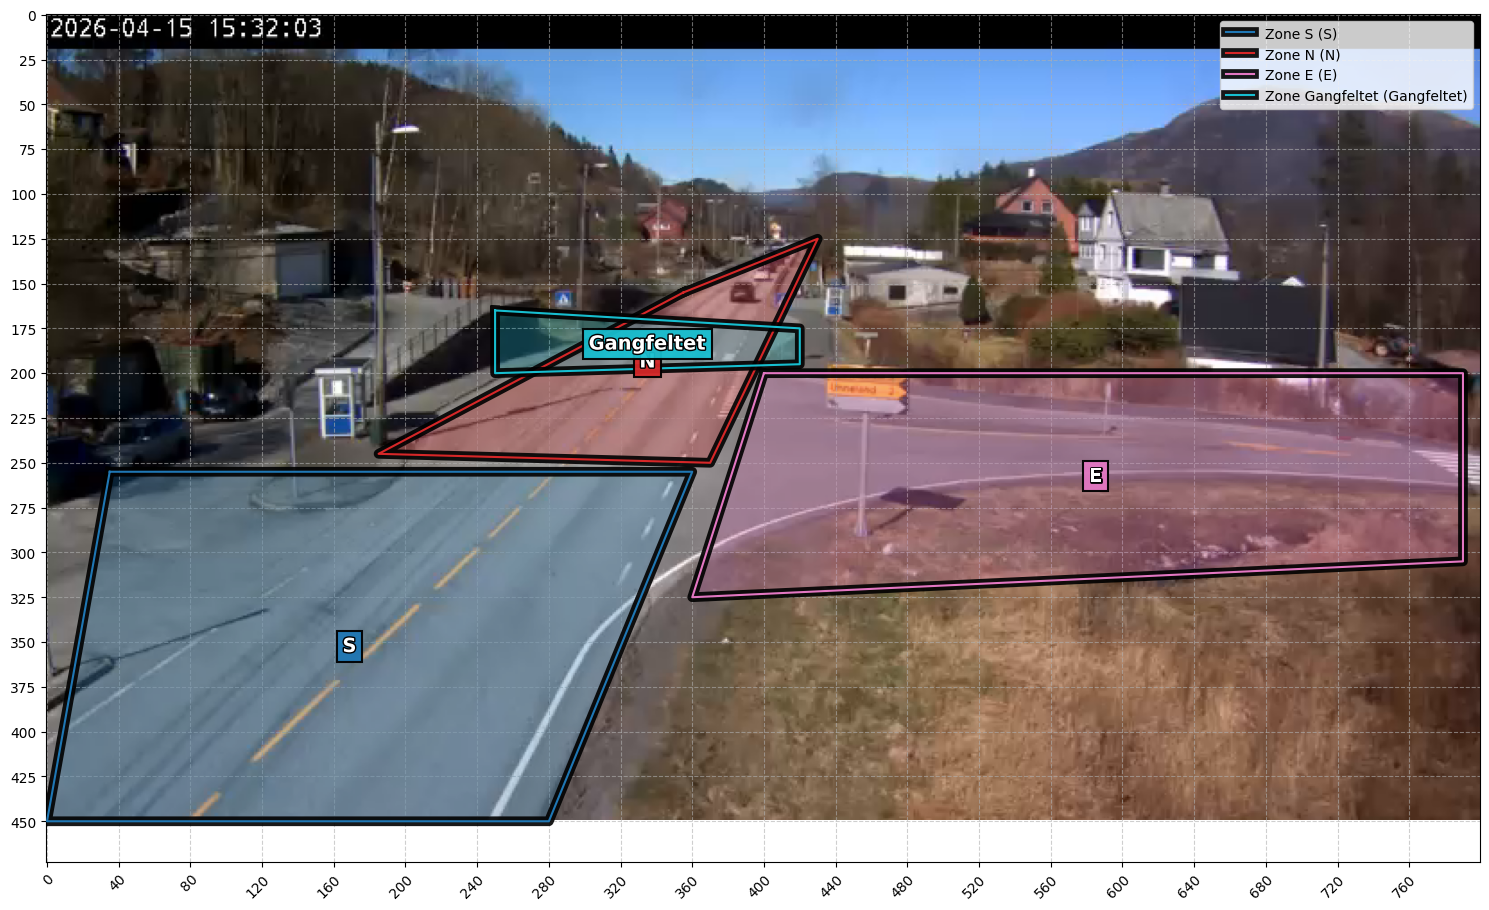
\includegraphics[width=0.9\linewidth]{project/images/Gatezones.png}
    \caption{Visualization of manually defined gate zones overlaid on a reference frame, including a coordinate grid used for calibration.}
    \label{fig:Gatezones}
\end{figure}

\subsection{Tracking Pipeline}
\label{sec:method_pipeline}

The full processing pipeline is implemented in the function \texttt{run\_video\_deploy}, which converts raw video into O--D outputs through the following steps as visualized in \autoref{fig:flow_tracking}:

\begin{figure}[H]
    \centering
    \includegraphics[width=1.0\linewidth]{project/images/flow_tracking.png}
    \caption{Tracking Pipeline}
    \label{fig:flow_tracking}
\end{figure}

\subsubsection{Video processing and ROI selection}
The input video is read using OpenCV, and metadata such as resolution, frame rate, and total frames are extracted. To reduce computational cost and avoid edge artifacts, tracking is performed only within a central region of interest (ROI), defined by horizontal and vertical ratios $(r_w, r_h)$. 

In addition, restricting the analysis to the central region improves classification reliability, as objects near the image boundaries are more prone to partial visibility, perspective distortion, and truncated bounding boxes, which can negatively affect both detection and classification performance.
\[
x_0=\left\lfloor\frac{(1-r_w)W}{2}\right\rfloor,\quad x_1=W-x_0,\quad
y_0=\left\lfloor\frac{(1-r_h)H}{2}\right\rfloor,\quad y_1=H-y_0.
\]
Each frame is cropped to this ROI prior to inference, while the ROI boundary is visualized in the output video.

\subsubsection{Dynamic Tracker Switching}
\label{sec:method_dynamic_switching}

To maintain robust tracking across varying lighting conditions (day, night, and twilight), the pipeline employs adaptive tracker selection based on real-time illumination analysis. The system automatically detects the current lighting condition and selects an appropriate tracker configuration.

Mode detection is based on HSV color saturation. The mean saturation of each frame is compared to a threshold (\texttt{sat\_threshold = 20.0}), where frames with \texttt{sat\_mean < sat\_threshold} are classified as nighttime. In the SVV video streams, the transition from day to night occurs abruptly, with the footage switching from full color to near-grayscale, resulting in a sharp drop in saturation. To reduce sensitivity to short-term fluctuations, saturation values are averaged over a rolling window of approximately 2 seconds before thresholding.

Figure~\ref{fig:saturation_transition} illustrates the saturation signal during a transition sequence, showing how the detected drop aligns with the stream’s day–night switch and triggers a corresponding change in tracking configuration.



\begin{figure}[H]
    \centering
    \includegraphics[width=1\linewidth]{project/images/saturation.png}
    \caption{Rolling HSV saturation (\texttt{sat\_mean}) over time for the 10-minute transition video, including the decision threshold and detected tracker switch points.}
    \label{fig:saturation_transition}
\end{figure}

To prevent tracker flickering during twilight transitions or lighting artifacts, mode changes are subject to a persistence requirement. The system only commits to a new mode after it has been consistently detected for 5 seconds. This hysteresis mechanism prevents transient lighting fluctuations from triggering unnecessary tracker switches while still allowing adaptation to sustained illumination changes.

When a mode switch is detected, the tracker is switched from the best day configuration to the best night configuration (or vice versa). In practice, some identities can split across the switch; these split IDs are handled in a dedicated post-processing step during finalization, described in Section~\ref{sec:method_split_id_recovery}.

\subsubsection{Detection and tracking}
A YOLO-based detector is executed in tracking mode with persistent identities. The tracker assigns a unique ID to each vehicle and maintains this identity across frames, enabling trajectory reconstruction and temporal analysis.

Each detected bounding box $(x_1,y_1,x_2,y_2)$ is reduced to a single representative point. Two alternatives are supported: the centroid and the bottom-center point. The bottom-center point,
\[
\left(\frac{x_1+x_2}{2},\,y_2-\delta\right),
\]
is used by default, as it better approximates the vehicle's position on the road plane and is less sensitive to perspective distortion.

A vehicle is considered inside a gate zone if its tracking point lies within the corresponding polygon. This is evaluated using a standard point-in-polygon test.

\subsubsection{Zone Stabilization and O--D Logic}
\label{sec:method_od_logic}

To avoid spurious transitions caused by detection noise near zone boundaries, zone assignments are stabilized using a dwell-time constraint. For each track $i$, a short history buffer of recent zone assignments is maintained:
\[
H_t(i) = [z_{t-K+1}(i), \ldots, z_t(i)],
\]
where $z_t(i)$ denotes the zone at frame $t$. A stable zone is declared if the last $K$ non-null entries are identical. In this study, $K=3$ frames (the default \texttt{zone\_dwell\_frames} parameter) is used as a compromise between responsiveness and robustness. Additionally, only tracks that have been active for at least \texttt{min\_track\_frames} are eligible for O--D counting, filtering out spurious detections (typically 5 frames in daytime experiments, and reduced to 2 frames in selected night/transition evaluations).

The O--D logic is defined as follows:
\begin{itemize}
    \item The first stable zone observed for a track defines its origin $o(i)$.
    \item The destination $d(i)$ is taken as the last stable zone observed for that track before finalization.
    \item Each track contributes at most one O--D event $o(i) \rightarrow d(i)$.
\end{itemize}

An O--D event is counted only when $o(i) \neq d(i)$ at finalization (e.g., when the track is inactive for the configured gap), which ensures that each vehicle is counted once and reduces overcounting from short-term boundary oscillations.

\subsubsection{Track-Level Class Stabilization}
\label{sec:method_class_stabilization}

To obtain robust vehicle classification, class predictions are aggregated over the lifetime of each track. For each track ID, both the predicted classes and their associated confidence scores are stored across frames.

For each class, the number of occurrences and the average confidence are computed. A class is considered stable if it appears in at least five frames. If one or more stable classes exist, the class with the highest average confidence is selected. Otherwise, the class that appears most frequently is chosen.

This approach reduces the impact of occasional misclassifications and provides more consistent class labels for O--D analysis.

\subsubsection{O--D Matrix Construction}
\label{sec:method_od_matrix}

O--D counts are aggregated by destination $d$, origin $o$, and vehicle class $c$:
\[
M_{d,o,c} \leftarrow M_{d,o,c} + 1.
\]
In addition to the aggregated matrix, an event log is maintained containing the frame index, track ID, origin, destination, class label, and confidence for each detected transition.

\subsubsection{Split ID Recovery}
\label{sec:method_split_id_recovery}
During extended video analysis, a single vehicle track may become fragmented into multiple identities. This can happen when the tracker switches between day and night configurations, but also when detections are interrupted by brief occlusions, low confidence, or other tracking gaps. Such fragmentation results in incomplete O--D trajectories and can cause undercounting. To mitigate this effect, a post-processing step reconstructs fragmented identities during finalization by matching compatible track fragments. As mentioned as a knowledge gap, occlusion is a frequent cause of such fragmentation and identity switches in MOT systems, yet handling it explicitly remains an open challenge in vehicle-tracking research \citep{Hassan2024}.

Track fragments are extracted from the detection history, with each fragment defined by its temporal interval (start and end frame), spatial positions (start and end points), dominant vehicle class, and an estimated velocity vector. The recovery step considers two types of cases: tracks that already contain a valid origin--destination transition but were not counted earlier, and pairs of fragments that may belong to the same vehicle across a gap. Candidate matches are evaluated using a multi-criteria cost function that penalizes:
\begin{itemize}
    \item \textbf{Spatial distance:} Euclidean distance between the end position of the earlier fragment and the start position of the later fragment, compared against a threshold (default: $\text{max\_dist\_raw} = 180$ pixels).
    \item \textbf{Velocity-predicted distance:} For fragments with sufficient temporal support, the expected continuation point is estimated using the fragment velocity. The distance between the predicted and observed start positions is compared against a stricter threshold (default: $\text{max\_dist\_pred} = 160$ pixels).
    \item \textbf{Class consistency:} Fragments with different dominant vehicle classes incur a penalty (default: $\text{class\_penalty} = 40$ pixels equivalent) to the distance metric, reducing but not preventing matches between visually distinct classes.
    \item \textbf{Temporal proximity:} Only fragments separated by a temporal gap of less than the threshold (default: $\text{max\_gap\_seconds} = 3$ seconds) are considered for matching.
\end{itemize}
Matches are resolved greedily by selecting the lowest-cost candidate that satisfies all constraints. Successfully matched fragments are merged into a single identity, while valid single-fragment trips that were missed earlier are added directly to the O--D counts. This improves the completeness of the trajectory set and the accuracy of the final O--D matrix.

\subsubsection{Outputs and Quality Control}
\label{sec:method_outputs}
The pipeline produces compact, machine-readable outputs and brief QC artifacts:
\begin{itemize}
    \item \textbf{Exports:} annotated video (MP4), event logs, trajectories (CSV/JSON), and full track dumps (pickle/JSON).
    \item \textbf{Tracking statistics:} processing time, achieved FPS, total detections, frames without track IDs, and a split-id summary.
    \item \textbf{Evaluation exports:} O--D matrices and summary metrics (class error, route error, total error, \% error)
    \item \textbf{Reproducibility metadata:} model version, tracker configurations, time for tracker switching, random seed, and run timestamp are recorded with outputs.
\end{itemize}

An example of the annotated output is shown in Figure~\ref{fig:tracking_output}. The figure illustrates how detected vehicles are represented with bounding boxes, track IDs, and class labels, as well as their trajectories over time. The region of interest (ROI) is highlighted. In addition, live current origin-destination counts are displayed.

\begin{figure}[H]
    \centering
    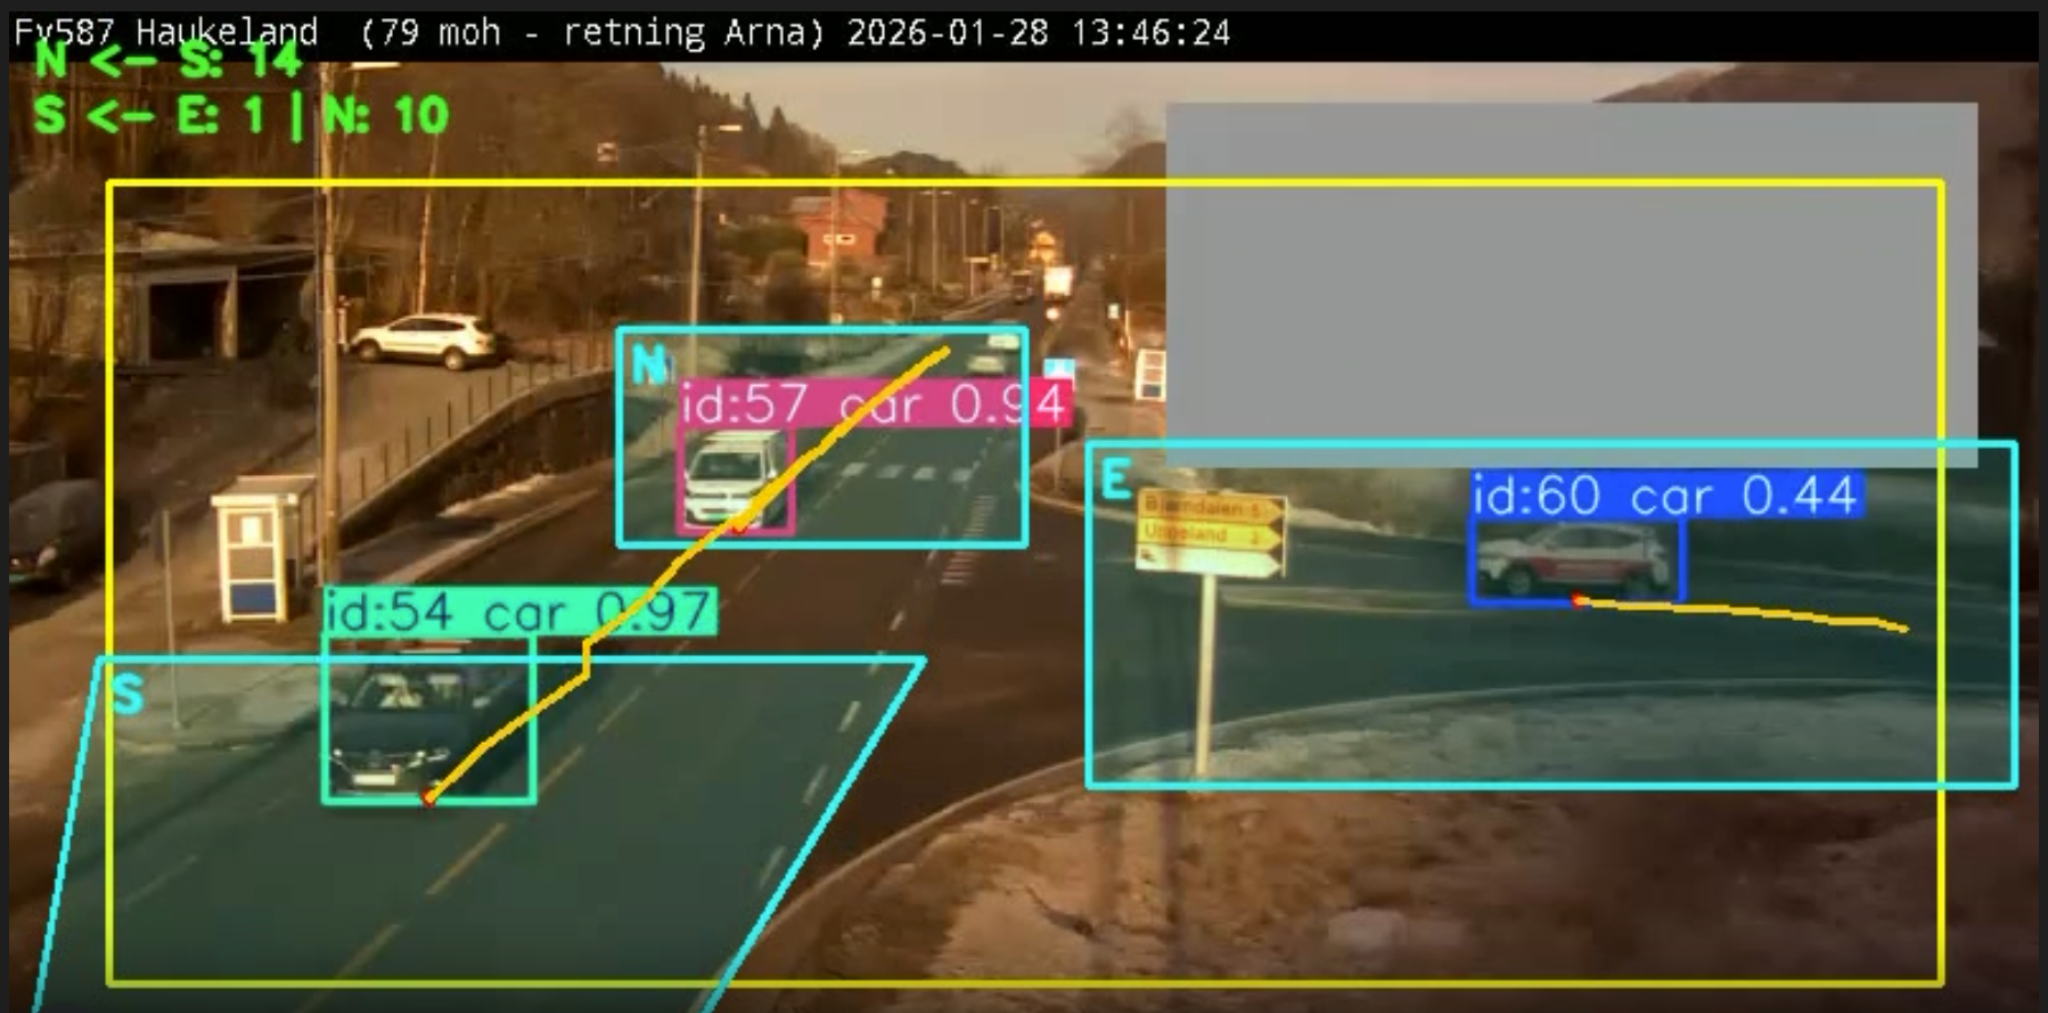
\includegraphics[width=0.9\linewidth]{project/images/tracking_output.png}
    \caption{Annotated tracking output showing detections, trajectories, gate zones, and O--D overlay.}
    \label{fig:tracking_output}
\end{figure}

\subsection{Experimental Design and Evaluation Protocol}
\label{sec:method_eval_protocol}

Tracking performance is evaluated end-to-end as a detection + tracking + zone-based origin--destination (O--D) aggregation pipeline. Two detectors (YOLO26n and YOLO26m) are combined with three tracking strategies, yielding six configurations per lighting condition: ByteTrack, default BoT-SORT, and a custom BoT-SORT profile tuned for the relevant time of day.

The evaluation follows a staged protocol:

\begin{enumerate}
    \item \textbf{Daytime screening (15 minutes):} six configurations are evaluated on a 15-minute daytime segment to compare detector capacity and tracker choice under normal lighting and to select the best-performing daytime setup.
    \item \textbf{Daytime validation (1 hour, rush-hour):} the selected best daytime configuration is evaluated on a 1-hour daytime rush-hour segment to assess performance stability over longer sequences.
    \item \textbf{Night-time evaluation (1 hour):} six configurations are evaluated on a 1-hour night-time segment. Night-time processing is faster due to the reduced frame rate of the video stream, making full comparison across configurations computationally feasible.
    \item \textbf{Day--night transition (10 minutes):} an additional twilight sequence is used to evaluate autonomous operation across changing lighting conditions, using dynamic switching between the day-optimized and night-optimized tracker configurations.
\end{enumerate}


%The proposed system is evaluated under four distinct experimental scenarios. First, all six model--tracker combinations are tested on a 15-minute daytime segment to assess baseline performance and compare configurations under controlled conditions. Second, the best-performing configuration from this stage is further evaluated on a 1-hour daytime rush-hour segment to assess temporal stability under increased traffic density.

%Third, all configurations are evaluated on a 1-hour night-time segment to assess robustness under low-light conditions. Finally, a 10-minute day--night transition sequence is used to evaluate system behavior under changing illumination, including the effectiveness of the dynamic tracker switching mechanism.